\documentclass[12pt,aspectratio=169]{beamer}

\usetheme{metropolis}

\definecolor{mDarkBrown}{HTML}{FF5722}
\definecolor{mDarkTeal}{HTML}{263238}
\definecolor{mLightBrown}{HTML}{FF5722}

\usepackage{booktabs}
\usepackage{graphicx}
\usepackage{hyphenat}
\usepackage{multirow}
\usepackage{nicefrac}
\usepackage[normalem]{ulem}

\usepackage{pifont}
\newcommand{\cmark}{\ding{51}}
\newcommand{\xmark}{\ding{55}}

\usepackage{minted}
\usemintedstyle{tango}
\newminted[bash]{bash}{%
    autogobble,
    bgcolor=mDarkTeal!10,
    linenos
}
\newminted[py3]{python}{%
    python3,
    autogobble,
    bgcolor=mDarkTeal!10,
    linenos
}
\newminted[sql]{sql}{%
    autogobble,
    bgcolor=mDarkTeal!10,
    linenos
}

\usepackage{polyglossia}
\setdefaultlanguage[variant=british]{english}
\usepackage[english=british]{csquotes}

\defaultfontfeatures{Ligatures=TeX}
\setmainfont{Lucida Sans OT}
\setsansfont[Scale=MatchLowercase]{Lucida Sans OT}
\setmonofont[Scale=MatchLowercase]{Lucida Console DK}

\usepackage{mathspec}
\setmathsfont(Digits,Latin,Greek)[Numbers={Lining,Proportional}]{Lucida Bright Math OT}

\newcommand{\mat}[1]{\ensuremath{\mathbf{#1}}}

\newcommand{\R}{\ensuremath{\mathbb{R}}}

\newcommand{\E}[1]{\ensuremath{\mathbb{E}\!\left[ #1 \right]}}
\newcommand{\V}[1]{\ensuremath{\mathbb{V}\!\left[ #1 \right]}}
\newcommand{\Prob}[1]{\ensuremath{\Pr\!\left( #1 \right)}}
\newcommand{\Normal}[2]{\ensuremath{\mathcal{N}\!\left( #1, #2 \right)}}
\newcommand{\simiid}{\ensuremath{\overset{\text{\tiny i.i.d.}}{\sim}}}

\DeclareMathOperator{\logit}{logit}

\author{Gianluca Campanella}
\date{}



\title{Introduction to prediction}

\begin{document}

\maketitle

\begin{frame}{Contents}
    \tableofcontents[hideallsubsections]
\end{frame}

\section{Prediction and loss functions}

\begin{frame}{Guessing values}
    \begin{itemize}
        \item $Y$ = `time it takes you to get to work in the morning'
        \item You have some realisations $y_{1}, y_{2}, \ldots$ collected over
              time
        \item You want to predict the value of $Y$ tomorrow
    \end{itemize}
    \vfill\pause
    \begin{center}
        {\Large%
         How do you do this?} \\[1em]
        {If you prefer, what's the \alert{optimal point forecast} for $Y$?}
    \end{center}
\end{frame}

\begin{frame}{Loss functions}
    Before you can answer, you need a \alert{loss function} that\ldots
    \begin{itemize}
        \item Measures how big an error you're making with your guess $g$
        \item Can be minimised to obtain the `best' $g$
    \end{itemize}
    \vfill\pause
    \begin{center}
        \renewcommand*{\arraystretch}{1.5}
        \begin{tabular}{ll}
            \toprule
            \textbf{Mean squared error}  & $\operatorname{MSE}(g) = \E{ (Y - g)^{2}}$ \\
            \textbf{Mean absolute error} & $\operatorname{MAE}(g) = \E{ |Y - g|}$ \\
            \bottomrule
        \end{tabular}
    \end{center}
\end{frame}

\begin{frame}{Towards prediction\ldots}
    Usually we have at least another variable $X$ that we believe to be related
    to $Y$\ldots
    \vfill\pause
    \begin{block}{Idea}
        Using some function $f$ of $X$, we should be able to predict $Y$
        `\alert{better}' (i.e.\ reduce the mean error) than by ignoring it
        \vfill
        \[
            g
            \;
            \rightarrow
            \;
            f(X)
            \quad
            \text{and thus}
            \quad
            \operatorname{MSE}(f\,) = \E{(Y - f(X))^{2}}
        \]
    \end{block}
\end{frame}

\begin{frame}[t]{What should $f$ be?}
    \only<1>{%
        Consider the decomposition
        \[
            Y\,|\,X = f^{\,\star}(X) + \epsilon
        \]
        \begin{itemize}
            \item $f^{\,\star}$ is the optimal prediction (conditional on knowing $X$)
            \item $\epsilon$ is a random variable (since $f^{\,\star}$ is not)
            \item $\E{\epsilon} = 0$ without loss of generality
        \end{itemize}}
    \only<2>{%
        For the MSE, it can be shown that
        \[
            f^{\,\star}(x) = \E{ Y\,|\,X = x }
        \]
        \vfill
        $f^{\,\star}$ is what we'd like to know when we want to predict $Y$
        given $X$
        \begin{flushright}
            \ldots but can we?
        \end{flushright}}
\end{frame}

\section{Bias\hyp{}variance trade\hyp{}off}

\begin{frame}[t]{Bias\hyp{}variance trade\hyp{}off}
    \only<1>{%
        Suppose that\ldots
        \begin{itemize}
            \item The `true' regression function is $f^{\,\star}$
            \item We have to make do with some suboptimal $f$
        \end{itemize}
        \vfill
        Let's start by expanding\ldots
        \begin{align*}
            (Y - f \,)^{2}
            &= ( Y - f^{\,\star} + f^{\,\star} - f \,)^{2} \\
            &= [ ( Y - f^{\,\star} ) + ( f^{\,\star} - f \,) ]^{2} \\
            &= ( Y - f^{\,\star} )^{2}
               + 2 ( Y - f^{\,\star} ) ( f^{\,\star} - f \,)
               + ( f^{\,\star} - f \,)^{2}
        \end{align*}}
    \only<2>{%
        Now take the expectation\ldots
        \[
            \E{( Y - f^{\,\star} )^{2}
               + 2 ( Y - f^{\,\star} ) ( f^{\,\star} - f \,)
               + ( f^{\,\star} - f \,)^{2}}
        \]
        \vfill
        Since $Y - f^{\,\star} = \epsilon$ and $\E{\epsilon} = 0$\ldots
        \begin{itemize}
            \item $\E{( Y - f^{\,\star} )^{2}} = \V{\epsilon}$
            \item $\E{Y - f^{\,\star}} = \E{\epsilon} = 0$
            \item $\E{( f^{\,\star} - f \,)^{2}} = ( f^{\,\star} - f \,)^{2}$ (non\hyp{}random)
        \end{itemize}}
    \only<3>{%
        \[
            \operatorname{MSE}(f\,) = \alert{\V{\epsilon}} + ( f^{\,\star} - f \,)^{2}
        \]
        \vfill
        \begin{block}{Variance $\V{\epsilon}$}
            \begin{itemize}
                \item Doesn't depend on $f$, just on `how hard' it is to predict
                      $Y\,|\,X = x$
                \item It's the unpredictable, irreducible fluctuation around
                      even the best prediction (randomness rules our lives!)
            \end{itemize}
        \end{block}}
    \only<4>{%
        \[
            \operatorname{MSE}(f\,) = \V{\epsilon} + \alert{( f^{\,\star} - f \,)^{2}}
        \]
        \vfill
        \begin{block}{Bias $( f^{\,\star} - f \,)^{2}$}
            \begin{itemize}
                \item It's the `extra error' we get from not knowing $f^{\,\star}$
                \item It's also the amount by which we are systematically off
            \end{itemize}
        \end{block}}
    \only<5>{%
        Since $f$ is itself estimated from a sample (it's actually $\hat{f}\,$),
        we have\ldots
        \begin{itemize}
            \item The \alert{irreducible variance} due to the stochastic process
            \item The \alert{bias} in approximating $f^{\,\star}$ using $f$
            \item The additional \alert{estimation variance} of $\hat{f}$
        \end{itemize}
        \vfill
        \begin{block}{Consistent methods}
            \begin{itemize}
                \item Bias and estimation variance $\to 0$ as the sample size
                      increases
                \item Different consistent methods may converge at different
                      rates
            \end{itemize}
        \end{block}}
    \only<6>{%
        \begin{center}
            \vfill
            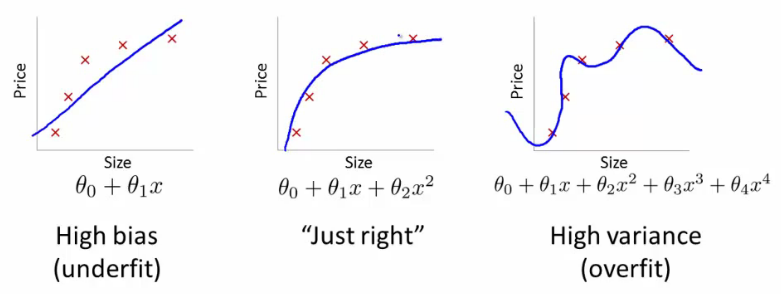
\includegraphics[width=\textwidth]{figures/underfitting_overfitting} \\[\bigskipamount]
            {\scriptsize%
             From Andrew Ng's \textit{Machine Learning} course}
            \vfill
        \end{center}}
\end{frame}

\section{Generalisability}

\begin{frame}{Bias\hyp{}variance trade\hyp{}off and generalisability}
    \begin{center}
        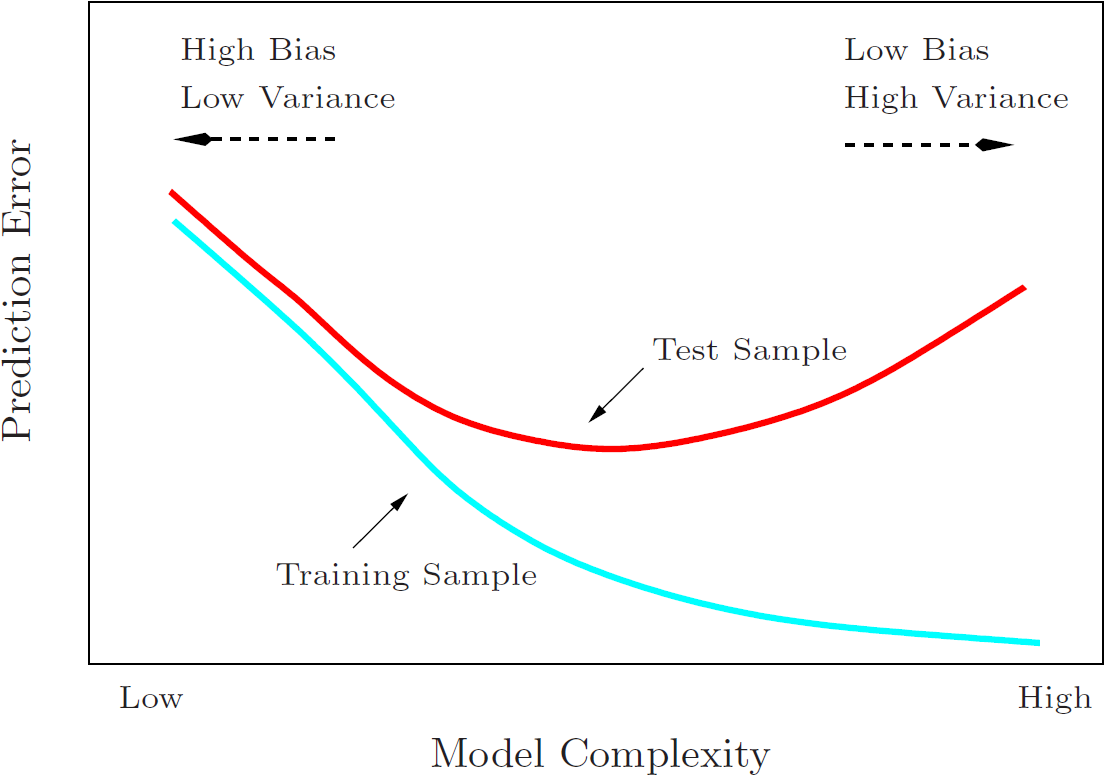
\includegraphics[height=0.8\textheight]{figures/generalisability} \\
        {\scriptsize%
         From \textit{The Elements of Statistical Learning}}
    \end{center}
\end{frame}

\begin{frame}{Cross\hyp{}validation}
    \begin{block}{General idea}
        \begin{itemize}
            \item Fit several models on subsets of the data
            \item Measure performance of each
            \item Compute the mean performance
        \end{itemize}
    \end{block}
\end{frame}

\begin{frame}{$k$-fold cross\hyp{}validation}
    \begin{itemize}
        \item Split the data into $k$ groups (a.k.a.\ `folds')
        \item Repeat for each fold:
              \begin{itemize}
                  \item Fit the model using all but the selected fold
                  \item Measure performance on the selected fold
              \end{itemize}
        \item Compute the mean performance across folds
    \end{itemize}
\end{frame}

\begin{frame}{Regularisation}
        \begin{itemize}
        \item Penalise `large' coefficients by shrinking them
        \item Helps avoid overfitting
        \item Requires \alert{tuning} of an additional parameter $\alpha$
              representing the `weight' of the penalty (relative to the
              prediction error)
    \end{itemize}
    \vfill
    \begin{center}
        \renewcommand*{\arraystretch}{1.5}
        \begin{tabular}{lll}
            \toprule
            $L_{1}$ & LASSO & $\sum_{j} | \beta_{j} |$ \\
            $L_{2}$ & Tikhonov or ridge & $\sum_{j} \beta_{j}^{2}$ \\
            \bottomrule
        \end{tabular}
    \end{center}
\end{frame}

\end{document}

